\section{Modeling \podtm} \label{sec:pod-model}
In this section, we introduce the notion of a \podtm, a distributed protocol where clients can \emph{read} and \emph{write} transactions.
We first define the basic data structures of a \podtm protocol.

\begin{definition}[Transaction trace and trace set]
    The \emph{transaction trace} of a transaction $\tx \in \zo^*$ is a tuple containing the values $(\tx, \rmin, \rmax, \rconf)$, which change during the execution of a \podtm protocol.
    We call $\rmin \in \BN$ the \emph{minimum round}, $\rmax \in \BN \cup \{\infty\}$ the \emph{maximum round},
    $\rconf \in \BN \cup \{\bot\}$ the \emph{\confirmed round}.
    We denote by $\rmax=\infty$ an unbounded maximum round and by $\rconf=\bot$ an undefined \confirmed round.
    We also denote these values as $\tx.\rmin, \tx.\rmax$, and $\tx.\rconf$.
    A \emph{trace set} $\txSet$ is a set of transaction traces $\{(\tx, \rmin, \rmax, \rconf) \mid \tx \in \zo^*\}$.
\end{definition}

\begin{definition}[Confirmed transaction]
    A transaction with confirmed round \rconf is called \emph{\confirmed} if $\rconf \neq \bot$, and \emph{unconfirmed} otherwise.
\end{definition}

% \begin{definition}[Trace set]
% A \emph{trace set} $\txSet$ is a set of traces $(\tx, \rmin, \rmax, \rconf)$. We say that a transaction $\tx$ \emph{appears} in $\txSet$ when $\exists (\tx, \rmin, \rmax, \rconf) \in \txSet$, otherwise we say that a transaction $\tx$ \emph{does not appear} in $\txSet$.
% \end{definition}


\begin{definition}[Pod data structure]
    A \emph{pod data structure} $\Pod$ is a tuple $(\txSet, \rperf)$, where \txSet is a trace set and \rperf is a round number called the \emph{past-perfect round}.
\end{definition}
We denote the components of a pod data structure as $\Pod.\txSet$ and $\Pod.\rperf$.
We write $\tx \in \Pod.\txSet$ if an entry $(\tx, \cdot, \cdot, \cdot)$ exists in $\Pod.\txSet$.
We remark that transactions in \txSet may be \confirmed on unconfirmed. Moreover, \rperf will be used to define a completeness property on \txSet (the \emph{past-perfection} property of \podtm).

\begin{definition}[Auxiliary data]
    We associate with a pod data structure $\Pod$ some auxiliary data \cert, which will be used to validate \Pod.
    The exact implementation of \cert is irrelevant for the definition of \podtm;
    however, it is helpful to mention that in \podtm-core it will be a tuple $\cert = (\ppcert, \alltxcert)$,
    where $\ppcert$ will be a \emph{past-perfection certificate} and \alltxcert a map from each transaction \tx in $\Pod.\txSet$ to a \emph{transaction certificate} \txcert for \tx.
    Both contain digital signatures.
\end{definition}

%We now define the \podtm protocol interface and associated concepts.
\begin{definition}[Interface of a \podtm]\label{def:podinterface}
A \podtm protocol has the following interface.
\begin{itemize}
    \item $\opwrite{\tx}$:
    % \item $\opwrite{\tx} \returns (\rmin, \rmax, \rconf, \txcert)$:
    It writes a transaction \tx to the \podtm.

    \item $\opreadall{} \returns (\Pod, \cert)$:
    It outputs a pod data structure $\Pod = (\txSet, \rperf)$ and auxiliary data \cert.
    % The second output is called an \emph{equivocation-evidence pod} and can be either $\bot$ or $\tilde{\Pod} = (\tilde{\txSet}, \tilde{\rperf}, \tilde{\ppcert})$.
\end{itemize}
\end{definition}
We say that a client \emph{reads the} \podtm when it calls \opread{}.
If $\tx$ appears in $\txSet$,
%$(\tx, \rmin, \rmax, \rconf, \txcert) \in \txSet$
 we say that the client \emph{observes} \tx and, if $\tx.\rconf \neq \bot$, we say that the client \emph{observes \tx as \confirmed}.

\begin{definition}[Validity function]
    Apart from its interface functions,
    a pod protocol also specifies a computable, deterministic, and non-interactive function \opValid{\Pod, \cert} that takes as input a pod data structure $\Pod$ and auxiliary data $\cert$ and outputs a boolean value. We say that a pod data structure $\Pod$ is \emph{valid} if $\opValid{\Pod, \cert} = \true$.
\end{definition}


% \begin{definition}[Past-perfect round]
% 	Given a set \txSet obtained by an honest client who reads the pod, a round \rperf is \emph{past-perfect} if,
% 	for any transaction $\tx$ that does not appear in $ \txSet$, no honest client will ever observe \tx as confirmed with $\tx.\rconf < \rperf$.
% \end{definition}

\begin{definition}[View of the \podtm]
    We call \emph{view of the} \podtm and denote by \podView{\client}{\round} the data structure returned by \opreadall{}, where \opreadall{} is invoked by client \client and the output is produced at round \round.
    We remark that \round denotes the round when \opreadall{} outputs, as the client may have invoked it at an earlier round.
    % We denote the components of a view as $\podView{\client}{\round}=(\podView{\client}{\round}.\txSet,
    % \podView{\client}{\round}.\rperf)$.
    % We write $\tx \in \podView{\client}{\round}$ if $\tx$ appears in $\podView{\client}{\round}.\txSet$.
\end{definition}

We now introduce the basic definition of a \emph{secure} \podtm protocol, as well as some additional properties (\emph{timeliness} and \emph{monotonicity}) that it may satisfy.

\begin{definition}[Secure \podtm]\label{def:podsec}
A protocol is a \emph{secure} \podtm if it implements the \podtm interface of Definition~\ref{def:podinterface} and specifies a validity function \opValid{}, such that the following properties hold.
\begin{description}
    \item[(Liveness) Completeness:]
    Honest clients always output a valid pod data structure.
    That is, if \opread{} returns $(\Pod, \cert)$ to an honest client, then $\opValid{\Pod, \cert} = \true$.

    \item[(Liveness) Confirmation within \parConf:]
	Transactions of honest clients become \confirmed after at most \parConf rounds.
	Formally, if an honest client $\client$ writes a transaction \tx at round \round,
    then for any honest client $\client'$ (including $\client=\client'$) it holds that $\tx \in \podView{\client'}{\round + \parConf}$ and $\tx.\rconf \neq \bot$.


	\item[(Liveness) Past-perfection within \parPerf:]
	Rounds become past-perfect after at most $\parPerf$ rounds.
	Formally,
    for any honest client \client and round $\round \geq \parPerf$, it holds that $\podView{c}{\round}.\rperf \geq \round - \parPerf$.
    % for any valid pod \Pod obtained at round \round, it holds that $\Pod.\rperf \geq \round - \parPerf$.

	\item[(Safety) Past-perfection:]
    A valid pod \Pod contains all transactions that may ever obtain a \confirmed round smaller than $\Pod.\rperf$. Formally,
	the adversary cannot output $(\Pod_1, \cert_1)$ and $(\Pod_2, \cert_2)$ to the network, such that $\opValid{\Pod_1, \cert_1} \land \opValid{\Pod_2, \cert_2}$ and there exists a transaction $\tx$ such that $(\tx, \rmin^1, \rmax^1, \rconf^1) \not\in \Pod_1.\txSet$ and $(\tx, \rmin^2, \rmax^2, \rconf^2) \in \Pod_2.\txSet$ and $\rconf^2 \neq \bot$ and $\rconf^2 < \Pod_1.\rperf$.

	\item[(Safety) Confirmation bounds:]
    \sloppy{
    The values $\rmin$ and $\rmax$ bound the \confirmed round that a transaction may ever obtain. Formally,
    the adversary cannot output $(\Pod_1, \cert_1)$ and $(\Pod_2, \cert_2)$ to the network, such that $\opValid{\Pod_1, \cert_1} \land \opValid{\Pod_2, \cert_2}$ and there exists a transaction $\tx$ such that $(\tx, \rmin^1, \rmax^1, \rconf^1) \in \Pod_1.\txSet$ and $(\tx, \rmin^2, \rmax^2, \rconf^2) \in \Pod_2.\txSet$ and $\rmin^1 > \rconf^2$ or $\rmax^1 < \rconf^2$.
    }

    % \oa{\item[(Safety) Censorship resistance:]}
	% If the adversary makes progress (outputs some past-perfect round), then it must output all transactions confirmed up that past perfect round, minus some propagation period of $X$.
	% Formally, there is a parameter $X$ such that,
    % if the adversary outputs $(\Pod, \cert)$ to the network with $\opValid{\Pod, \cert}$, then \Pod contains all transaction with confirmed round $\rconf \geq \Pod.\rperf - X$.
    % \oa{This is not exactly true, the adversary may see a transaction with $\alpha - \beta$ votes. It would be true if the confirmation threshold was $\alpha  - \beta$. What is its connection with the past-perfection safety property?}
\end{description}
\end{definition}


%The \emph{confirmation within \parConf} property gives us that, if an honest client writes a transaction \tx, then \tx will obtain $\rconf \neq \bot$ within \parConf rounds, but it does not tell us \emph{what} that \rconf will be.
%Similarly,
The \emph{confirmation bounds} property gives $\rmin^1 \leq \rconf^2 \leq \rmax^1$, for $\rmin^1, \rmax^1, \rconf^2$ computed by honest clients, but it does not guarantee anything about the values of $\rmin^1$ and $\rmax^1$ (for example, it could trivially be $\rmin^1=0$ and $\rmax^1=\infty$).
To this purpose we define an additional property of \podtm, called \emph{timeliness}.
% , which can be satisfied along with the standard safety and liveness properties of \podtm.
Previous work has observed a similar property as orthogonal to safety and liveness~\cite{EPRINT:TziSriZin23}.

\begin{definition}[\podtm \parTemp-timeliness for honest transactions]\label{def:pod-timely}
    A \podtm protocol is \emph{\parTemp-timely} if it is a secure \podtm, as per Definition~\ref{def:podsec}, and for any honest clients $\client_1,\client_2$, if $\client_1$ writes transaction \tx in round $\round$ and $\client_2$ has view $\podView{\client_2}{\round'}$ in round $\round'$, such that $(\tx, \rmin, \rmax, \rconf) \in \podView{\client_2}{\round'}.\txSet$, then:\\
    % (observe that, from the \emph{confirmation within \parConf} property, \tx will become confirmed):
    % \begin{enumerate}
        (1) $\rconf \in (\round, \round + \parTemp]$;
        (2) $\rmax \in (\round, \round + \parTemp]$;
        (3) $\rmax - \rmin < \parTemp$, implying $\rmin \neq 0$ and $\rmax \neq \infty$.
    % \end{enumerate}
\end{definition}


Moreover, a \podtm protocol allows \rmin, \rmax, \rconf to change during an execution -- for example, clients in construction \podtm-core will update them when they receive votes from replicas.
In the full version of this paper~\cite[Appendix A]{DBLP:journals/corr/abs-2501-14931} we define \emph{monotonicity} properties that impose restrictions on how these values evolve.

We conclude this section with some visual examples in Figures \ref{fig:temperature} and \ref{fig:example-output}.
% \begin{figure}[h]
%     \centering
%     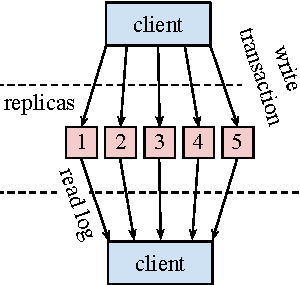
\includegraphics[width=0.35\textwidth]{figures/pod-architecture.pdf}
%     \caption{\todo{Add figure} }
%     \label{fig:example-output}
% \end{figure}


\begin{figure}[ht]
    \begin{minipage}[b]{.48\textwidth}
    \centering
    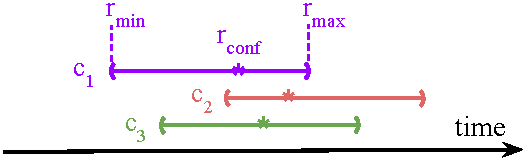
\includegraphics[width=1\textwidth]{figures/pod-temperature.pdf}
    \caption{The same transaction in the view of three different pod clients. Each client assigns it a minimum round \rmin and a maximum round \rmax. If it gets confirmed, the confirmation round \rconf will be
     between these two values. The \rconf that each client locally computes respects the bounds of each other client.}
     \label{fig:temperature}
    \end{minipage}
    \hfill
    \begin{minipage}[b]{.49\textwidth}
    \centering
    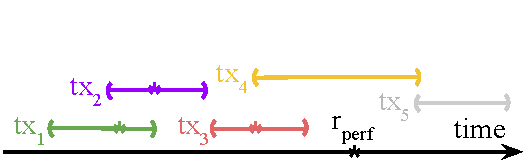
\includegraphics[width=1\textwidth]{figures/pod-example.pdf}
    \caption{A possible view of a single pod client.
    Transactions $\tx_1, \tx_2, \tx_3$ are confirmed, $\tx_4$ is not yet confirmed.
    A client also derives a past-perfect round $\rperf$. No transaction other than $\tx_1, \tx_2, \tx_3, \tx_4$ may  obtain $\rconf \leq \rperf$. There may exist $\tx_5$ for which the client has not received votes, but $\tx_5$ cannot obtain $\rconf \leq \rperf$.
    % Transactions written concurrently, or close to each other, such as $\tx_3$ and $\tx_4$, may not be totally ordered. Transactions written by malicious clients, such as $\tx_5$ may not become confirmed.
    }
    \label{fig:example-output}
    \end{minipage}
\end{figure}



% \subsection {Properties recap}
% This is for us. It summarizes the aforementioned properties and shows which algorithms satisfy them.
% \begin{center}
%     \begin{tabular}{ |l|c|c||c|c|c| }
%         \hline
%                                                                & \multicolumn{2}{c||}{streaming} & \multicolumn{2}{c|}{streaming+gossip}\\
%         \hline
%                                                                & sync  & async  &sync & async \\
%         Confirmation                                           & O& O& O& O\\
%         Pp liveness                                            & O& O& O& O\\
%         Common subset                                          & X& X& O& O\\
%         Common subset for honest tx                            & O& O& O& O\\
%         Conf. stickiness                                       & O& O& O& O\\
%         Correctness of assoc. values                           & O& O& O& O\\
%         Pp correctness                                         & O& O& O& O\\
%         Pp stickiness                                          & O& O& O& O\\
%         \hline
%     \end{tabular}
%     \end{center}
